\documentclass[10pt]{beamer}
\usepackage{makecell}
\usepackage{amssymb,amsmath}
\usepackage{graphicx}
\usepackage{url}
\usepackage{color}
\usepackage{pagenote}[continuous,page]
\usepackage{relsize}		% For \smaller
\usepackage{url}			% For \url
\usepackage{epstopdf}	% Included EPS files automatically converted to PDF to include with pdflatex

%For MindMaps
% \usepackage{tikz}%
% \usetikzlibrary{mindmap,trees,arrows}%

%%% Color Definitions %%%%%%%%%%%%%%%%%%%%%%%%%%%%%%%%%%%%%%%%%%%%%%%%%%%%%%%%%
%\definecolor{bordercol}{RGB}{40,40,40}
%\definecolor{headercol1}{RGB}{186,215,230}
%\definecolor{headercol2}{RGB}{80,80,80}
%\definecolor{headerfontcol}{RGB}{0,0,0}
%\definecolor{boxcolor}{RGB}{186,215,230}

%%% Save space in lists. Use this after the opening of the list %%%%%%%%%%%%%%%%
%\newcommand{\compresslist}{
%	\setlength{\itemsep}{1pt}
%	\setlength{\parskip}{0pt}
%	\setlength{\parsep}{0pt}
%}

%\setbeameroption{show notes on top}

% You should run 'pdflatex' TWICE, because of TOC issues.

% Rename this file.  A common temptation for first-time slide makers
% is to name it something like ``my_talk.tex'' or
% ``john_doe_talk.tex'' or even ``discrete_math_seminar_talk.tex''.
% You really won't like any of these titles the second time you give a
% talk.  Try naming your tex file something more descriptive, like
% ``riemann_hypothesis_short_proof_talk.tex''.  Even better (in case
% you recycle 99% of a talk, but still want to change a little, and
% retain copies of each), how about
% ``riemann_hypothesis_short_proof_MIT-Colloquium.2000-01-01.tex''?

\mode<presentation>
{
  \usetheme{CambridgeUS}
  \usecolortheme{dolphin}
  \useoutertheme{default}
  \useinnertheme{default}
  \setbeamercovered{invisible} % or whatever (possibly just delete it)
}
\beamertemplatenavigationsymbolsempty

\usepackage[english]{babel}
%\usepackage[latin1]{inputenc}
\usepackage{subfigure}

\usepackage{times}
\usepackage[T1]{fontenc}
\usepackage{CJKutf8}

%% makes the ppagenote command for figure references at the end.
\makepagenote
\renewcommand{\notenumintext}[1]{}
\newcommand{\ppagenote}[1]{\pagenote[Page \insertframenumber]{#1}}

\title[Experiment Design (01CH740)]{Experiment Design for Computer Sciences (01CH740)}
\author[Claus Aranha]{Claus Aranha\\{\footnotesize caranha@cs.tsukuba.ac.jp}}
\institute[U. Tsukuba]{University of Tsukuba, Department of Computer Sciences}



% TODO: this class needs more real examples from real data.


\title[]{Experiment Planning and Design}
\subtitle[]{Lecture 8: Course review and Scientific Communication}
\author[Claus Aranha]{Claus Aranha\\{\footnotesize caranha@cs.tsukuba.ac.jp}}
\institute{Department of Computer Science}
\date{2015-06-23}

\begin{document}

\section{Introduction}
\subsection{Introduction}
\begin{frame}
  \maketitle
\end{frame}

\section{Course review}
\subsection{Course Review}

\begin{frame}
  \frametitle{Class 1: What is Science}
  \begin{itemize}
  \item Method to learn more about the world
    \begin{itemize}
    \item ``Quest for truth''
    \item Social implications
    \end{itemize}
  \item Scientific and Unscientific Questions
  \item Scientific Method and Scientific Community
  \item Science vs Engineering
  \item Science vs Theory
  \item Computer Science
  \end{itemize}
\end{frame}

\begin{frame}
  \frametitle{Class 2: Experimental Science Concepts}
  \begin{itemize}
  \item What is an experiment: A methodical way to obtain facts about
    the world
  \item Experimental Factors - controllable and uncontrollable
    variation;
  \item Goals and Methodologies of an experiment;
  \item Types of experiment:
    \begin{itemize}
      \item Historical
      \item Observation
      \item Controlled
    \end{itemize}
  \item Experimental Rigour and Experimental reproducibility;
    \begin{itemize}
    \item Fairness
    \item Clarity
    \item Completeness
    \end{itemize}
  \end{itemize}
\end{frame}

\begin{frame}
  \frametitle{Class 3: Point and Interval Estimators}
  \begin{itemize}
  \item Experimental Data can be seen as a distribution\\
    (Sample vs Population)
  \item \structure{Point Estimators}: functions that describe this
    population;
    \begin{itemize}
    \item Examples: Mean, Median, Variance, Skew
    \item Point Estimators have their own distributions, variances, etc.
    \end{itemize}
  \item \structure{Interval Estimators}: Estimate the range of values
    produced by a point estimator;
    \begin{itemize}
    \item Confidence Interval;
    \item Prediction Interval;
    \item How to calculate these;
    \end{itemize}
  \item In general we want to describe our data as intervals, because
    it includes the value of a point estimator, and a prediction of
    how much it can vary;
  \item The role of the \structure{Central Limit Theorem}
  \end{itemize}
\end{frame}

\begin{frame}
  \frametitle{Class 4: Hypothesis testing for one Mean}
  \begin{itemize}
  \item Hypothesis testing as a mean to draw conclusions from data
  \item How to formulate a \structure{Null Hypothesis} and an \structure{Alternative Hypothesis}
  \item Hypothesis as statements about probabilities ($\alpha$, p, critical values)
  \item Hypothesis over the mean of a population
  \item \structure{The Student T Test}
  \item Assumptions of the T-test: Normality, Variance, Independence of Residuals;
  \item Errors Type I and Type II
  \end{itemize}
\end{frame}

\begin{frame}
  \frametitle{Class 5: Special cases of Hypothesis testing I}
  \begin{itemize}
  \item Paired Design;
  \item Non-parametric testing;
  \item Testing on the difference of two means;
  \item Proportion Testing
  \item Calculating $\alpha$, $\beta$ and sample size;    
  \end{itemize}
\end{frame}

\begin{frame}
  \frametitle{Class 6: Special cases of Hypothesis testing II}
  \begin{itemize}
  \item Multiple samples and ANOVA;
  \item Experimental Models;
    \begin{itemize}
      \item Completely Randomized Model and the Latin Hypercube
      \item Blocking Model
      \item Factorial Model
    \end{itemize}
  \end{itemize}
\end{frame}

\section{Case Studies}

\begin{frame}
  \frametitle{Case Studies}
  Let's see how these concepts fit together in two case studies
\end{frame}

\subsection{UFRJ Case Study}

\begin{frame}
  \frametitle{Case 1: Comparison of Drilling Riser Configuration}
  files/CS04.pdf
\end{frame}

\begin{frame}
  \frametitle{Case 1: Comparison of Drilling Riser Configuration}
  \begin{block}{How to approach this problem?}
    \begin{itemize}
    \item Question of interest 1: Is there a riser configuration (from
      options A, B, C) with a higher Meant Time to Failure (MTTF) than
      the standard configuration?
    \item Question of interest 2: If the answer to the question of
      interest 1 is YES, which configuration option has the highest
      Mean Time to Failure?
    \end{itemize}
  \end{block}
  \begin{block}{Main Concerns}
    \begin{itemize}
    \item Testing a riser configuration is expensive. The standard
      configuration has historical measures recorded, but each new
      observation will cost us money.
    \item Therefore, it is important to calculate beforehand the
      minimum number of observations that will be required.
    \end{itemize}
  \end{block}
\end{frame}

\begin{frame}
  \frametitle{Case 1: Comparison of Drilling Riser Configuration}
  \begin{block}{What tests to execute?}
    \begin{itemize}
    \item Because we are interested in the differences between
      multiple treatments, we initially need an ANOVA test to find out
      if they are different at all.
    \item If the ANOVA test indicates a significative difference
      between the treatments, a follow up ``all versus one'' test
      would tell us which treatments are better than the standard.
    \end{itemize}
  \end{block}
  
  \bigskip
  
  \begin{itemize}
  \item Because of the cost associated with each observation, we need
    to calculate in advance the sample sizes needed for the ANOVA and
    for the All versus One tests.
  \item This calculation can be done based on the required values for
    $\alpha$, $\beta$ and $\gamma$.
  \end{itemize}
\end{frame}

\begin{frame}[singleslide,fragile]
  \frametitle{Case 1: Comparison of Drilling Riser Configuration}
  
\begin{verbatim}
> model <- aov(LogTTF-Riser,data=yriser)
> summary.aov(model)

                   Df Sum Sq Mean Sq F value Pr (>F)
Riser               3   0.33  0.1108   0.439  0.725
Residuals         248  62.51  0.2521   
\end{verbatim}

\begin{center}
  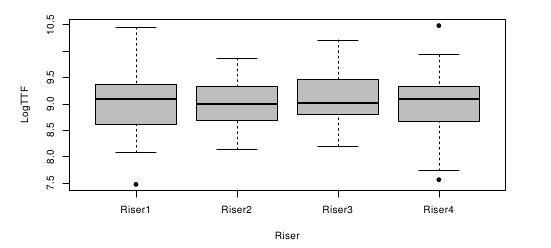
\includegraphics[width=0.8\textwidth]{fig/riser_result}
\end{center}

\medskip

The ANOVA test tells us that the risers do not significantly differ
from the standard configuration. Before we can accept this result and
end the experiment here, we need to validate this result.

\bigskip

\begin{itemize}
\item Shapiro-Wilk to test the normality of the data;
\item Fligner-Killeen to test that the variances of each group are homogeneous;
\item Durbin-Watson to test the lack of auto-correlation of the data;
\end{itemize}

\end{frame}

\section{Scientific Communication}
\subsection{After the experiment}
\begin{frame}
  \frametitle{Scientific Communications}
  
  \begin{center}
    Your science is only as useful as how many people know about it.
  \end{center}

  \bigskip

  So how do we make sure our results are actually used by other people?

  \smallskip

  \alert{Clarity}
\end{frame}

\begin{frame}
  \frametitle{What do we mean by clarity?}
  \begin{itemize}
  \item Experiment Clarity
  \item Paper Clarity
  \item Research Clarity
  \end{itemize}
\end{frame}

\begin{frame}
  \frametitle{Experiment Clarity}

  \begin{itemize}
  \item Is the experiment \structure{reproducible}? (big one)
  \item Is the data clear and available?
    \begin{itemize}
    \item Artificial Data;
    \item Real Data;
    \item Benchmark Data;
    \end{itemize}
  \item Are the conclusions clear?
  \end{itemize}

  \bigskip

  How do we write an experimental section of a paper to ensure clarity?
\end{frame}

\begin{frame}
  \frametitle{Paper Clarity}
  \begin{itemize}
  \item Beginning from the basics: Do not forget the spell checker!
  \item Have other people proofread your paper (regardless of the language)
  \item Follow the templates (unless you have a VERY good reason not to)
  \end{itemize}
\end{frame}

\begin{frame}
  \frametitle{Research Clarity}
  How organized is your research?
  \begin{itemize}
    \item Keeping a research diary
    \item Research Versioning (vs software versioning)
    \item Keep old versions of your experiment around!
  \end{itemize}
\end{frame}

\begin{frame}
  \frametitle{Reasons for clarity}

  In Medical sciences, it was found that over 80\% of the results were
  not reproducible after 20 years...
  
  \bigskip

  I don't wanna think about this proportion in computer sciences.
\end{frame}

\section{Ethical Considerations}
\subsection{Plagiarism}
\begin{frame}
  \frametitle{Plagiarism}
  \begin{itemize}
    \item Basic Plagiarism
    \item Small Plagiarism (figures, data, quotes, etc)
    \item Self-plagiarism
  \end{itemize}
\end{frame}

\subsection{Fraud}
\begin{frame}
  \frametitle{Fraud}
  \begin{itemize}
    \item How to avoid fraud by keeping your data open
    \item Taking care with claims
    \item Taking care with data and results
  \end{itemize}
\end{frame}

\subsection{Ethical Experiments}
\begin{frame}
  \frametitle{Experimenting with people}
  \begin{itemize}
    \item Molchan Experiment
    \item Stanford Prison Experiment
    \item Facebook Experiment
  \end{itemize}
\end{frame}

\section{Conclusion}

\subsection{Final Report}
\begin{frame}
  \frametitle{Final Report}
  \begin{block}{Important Dates:}
    \begin{itemize}
    \item June 30th (Tue): Question Class - make questions about your report here!
    \item July 7th (Tue): Final reports due!
    \end{itemize}
  \end{block}
  \begin{block}{Final Report Format}
    Upload a Zip file to manaba that include the following files:
    \begin{itemize}
    \item PDF file with your report, including the description of the
      research, the relevant experimental question, the experimental
      design, results etc (see the case study in this slides for info)
    \item R file with the code for any and all calculations that you
      did in your report.
    \item Any data files used in your calculations.
    \end{itemize}
  \end{block}
\end{frame}

\begin{frame}
  \frametitle{Final Report - Extra information:}
  \begin{block}{Format}
    There is no fixed format, but please remember that I want a well
    written pdf file. A suggestion for a report template is uploaded
    to Manaba.
  \end{block}
  \begin{block}{Case Studies}
    If you cannot use your own research/data for the final report, I
    have uploaded two case studies to Manaba. Choose one of those for
    your final report instead.
  \end{block}
\end{frame}

\subsection{Parting Words}

\begin{frame}
  \frametitle{Required Reading!}
  \begin{center}
    ``Experimental Computer Science: The Need for a Cultural Change''\\
    Dror G. Feitelson
  \end{center}

  \bigskip

  \url{http://www.cs.huji.ac.il/~feit/papers/exp05.pdf}
\end{frame}

\begin{frame}
  \frametitle{End of this class!}

  \begin{itemize}
  \item Let's take some time to do the course evaluation. 
  \item Questionnaries in English and Japanese are available
  \end{itemize}

  \begin{block}{Next Class}
    Questions and Report checking!
  \end{block}

\end{frame}


\end{document}
